\documentclass{beamer}
\setbeamercolor*{title}{fg=black}
\setbeamercolor*{frametitle}{fg=black}
\usepackage{graphicx}
\usepackage{polyglossia}
\setmainlanguage{russian}
\setmainfont{Times New Roman}
\setsansfont{Times New Roman}


\addtobeamertemplate{frametitle}{}{%
	\begin{picture}(0,0)
		\put(280,10){
\includegraphics[scale=0.05]{images/logo_osnovnoy_russkiy_chernyy.png}}
	\end{picture}
}
%Information to be included in the title page:
\title[About Beamer] %optional
{Польша в межвоенный период: 1918-1939 гг.}


\author{Сиромашенко Владислав Романович}

\institute[VFU] % (optional)
{
	Факультет программнрой инженерии и компьютерной техники\\
	Университет ИТМО
}

\date[VLC 2026] % (optional)
{Март 2026}



\begin{document}
	
	\frame{\titlepage}
	\begin{frame}
		\frametitle{\textbf{Ситуация}}
		
		\begin{columns}[T] 
			\column{0.5\textwidth}
			Падение трех империй:
			\begin{itemize}
				\item Германской
				\item Австро-Венгерской
				\item Российской
			\end{itemize}
			
			\column{0.5\textwidth}
			\centering
			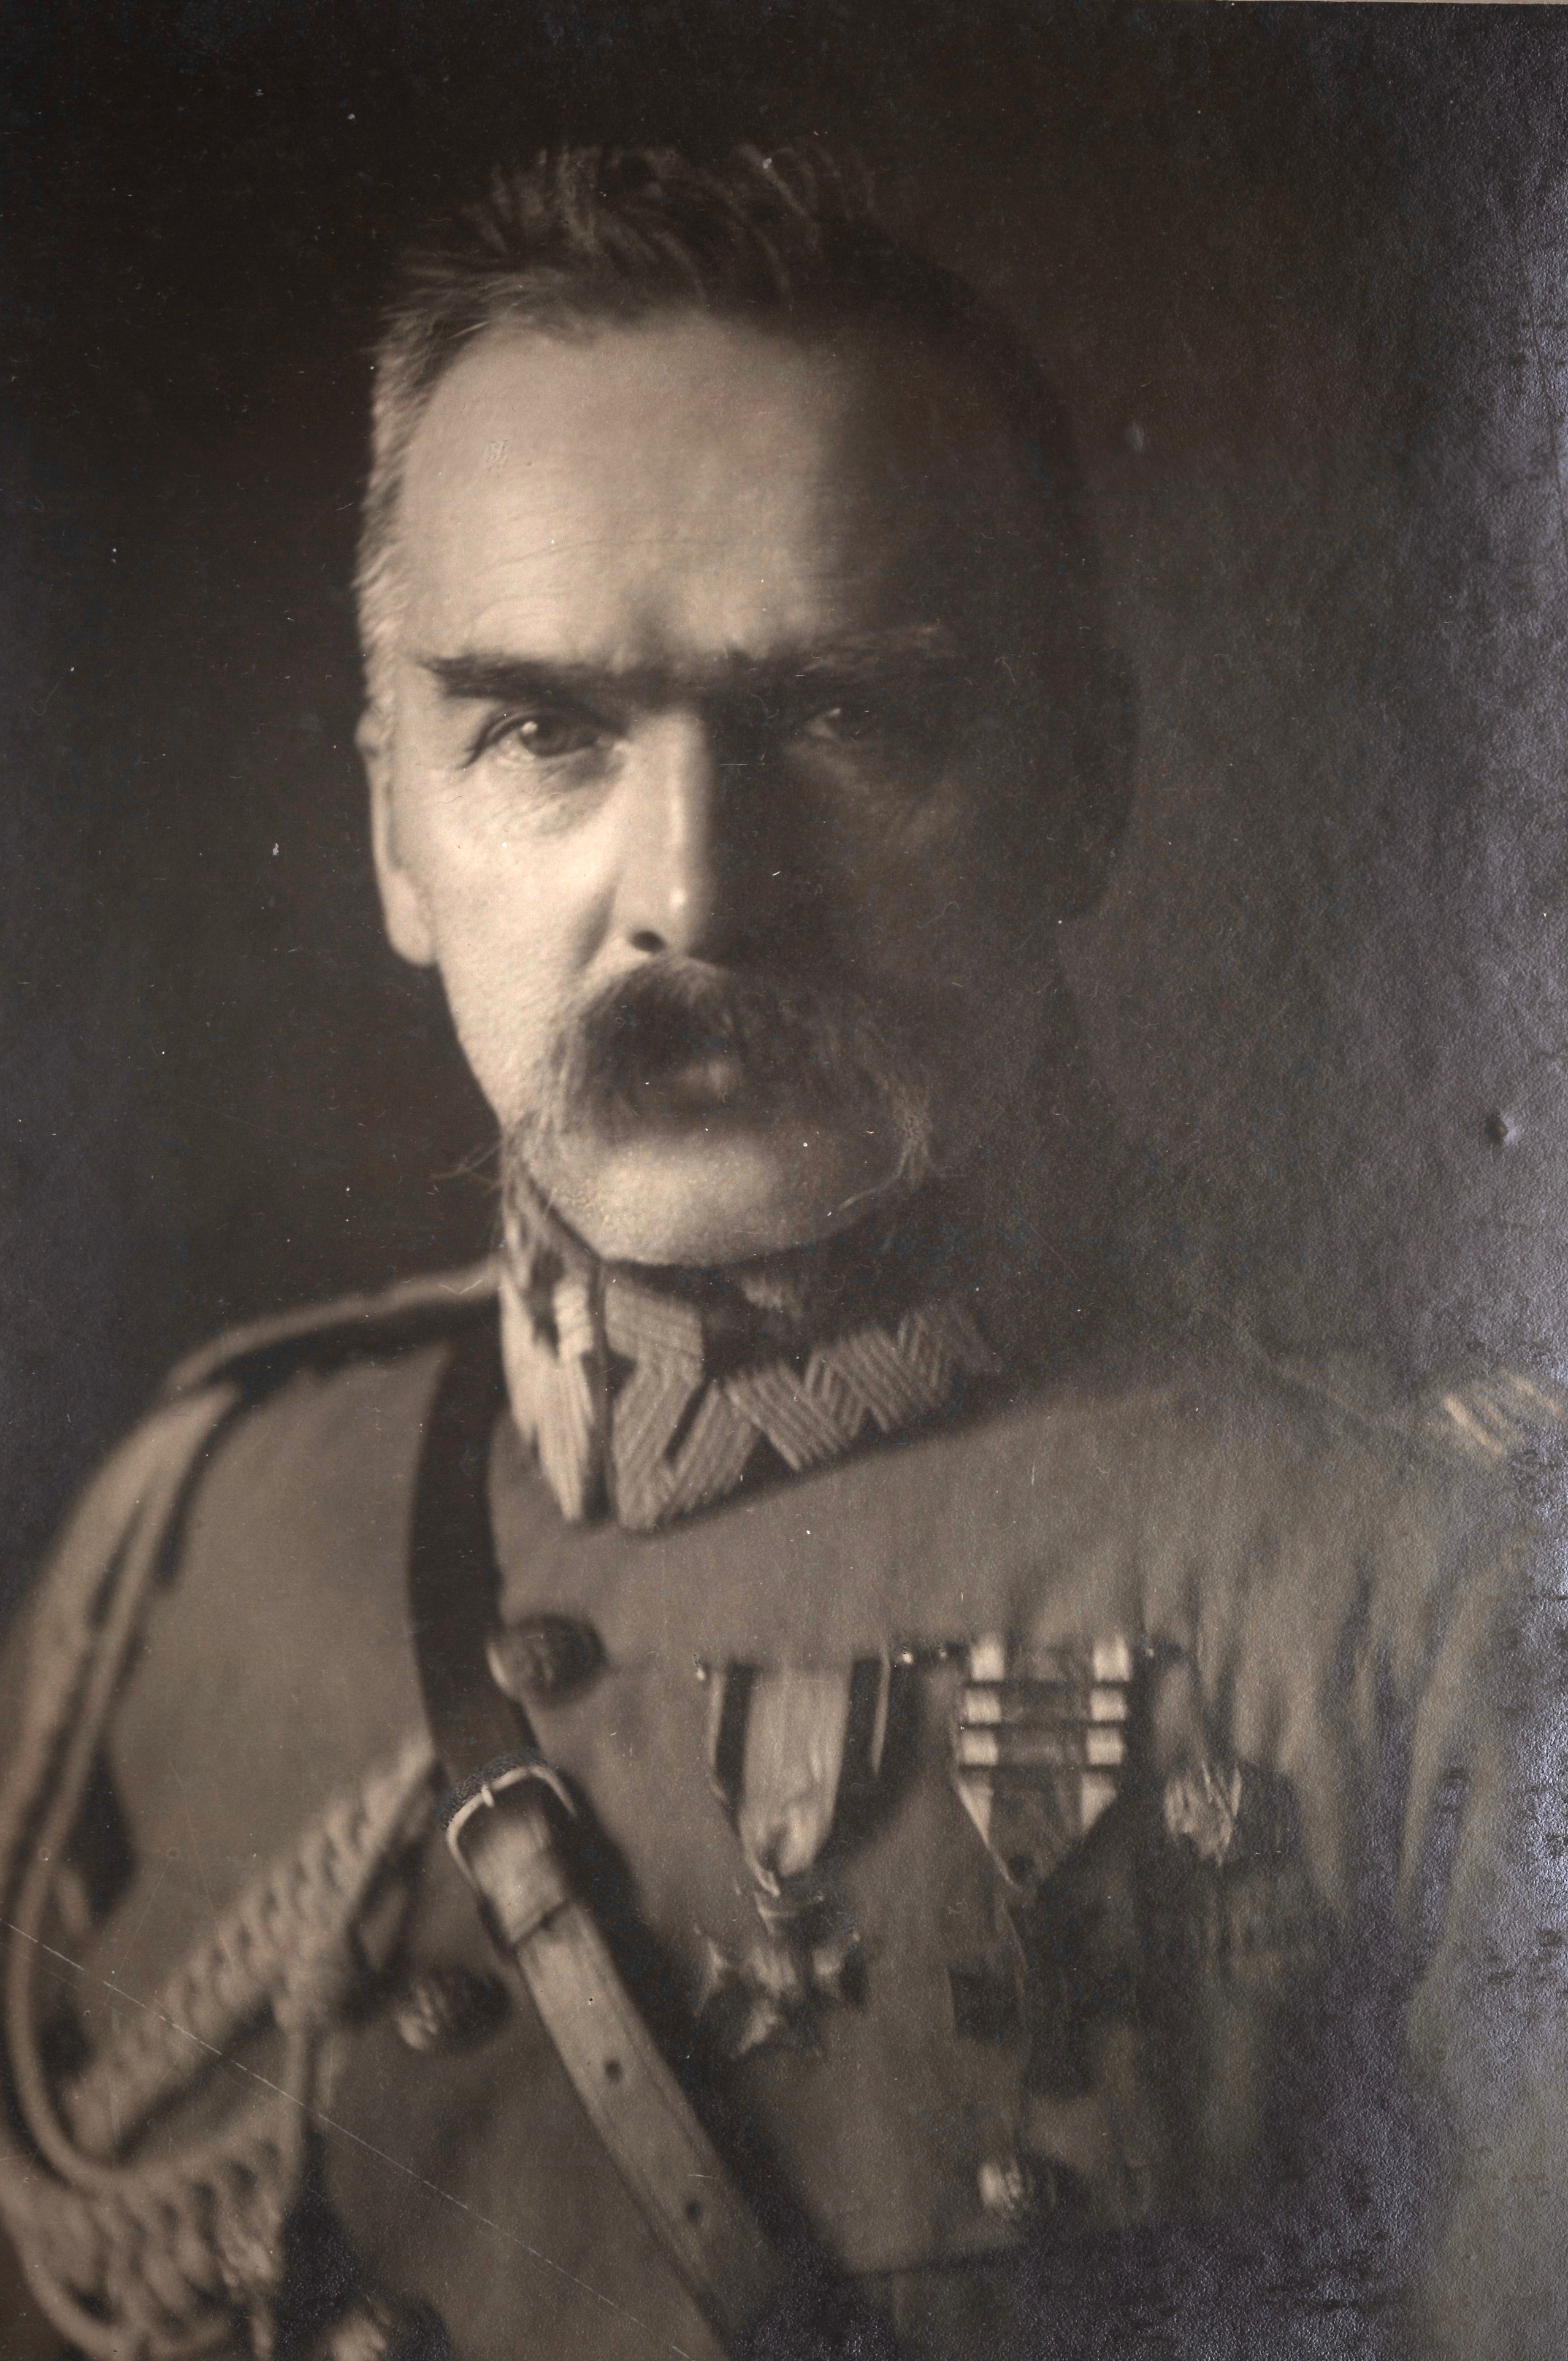
\includegraphics[width=0.8\textwidth]{images/Jozef_Pilsudski1.jpg}
			
			Ю́зеф Кле́менс Пилсу́дский \\
			\small{5 декабря 1867 — 12 мая 1935}
		\end{columns}
	\end{frame}
	
	
	\begin{frame}
		\frametitle{\textbf{Определение границ}}
		\begin{itemize}
			\begin{columns}[T] 
				\column{0.5\textwidth}
				\item Великопольское восстание \newline (Германия)
				\item Спор за тешинскую Силезию \newline (Чехословакия)
				\item Вильнюс \newline (Литва)
				\item Львов \newline (Заподно-украинская республика)
				\item Советско-польская война \newline (РСФСР)
				
				\column{0.5\textwidth}
				\centering
				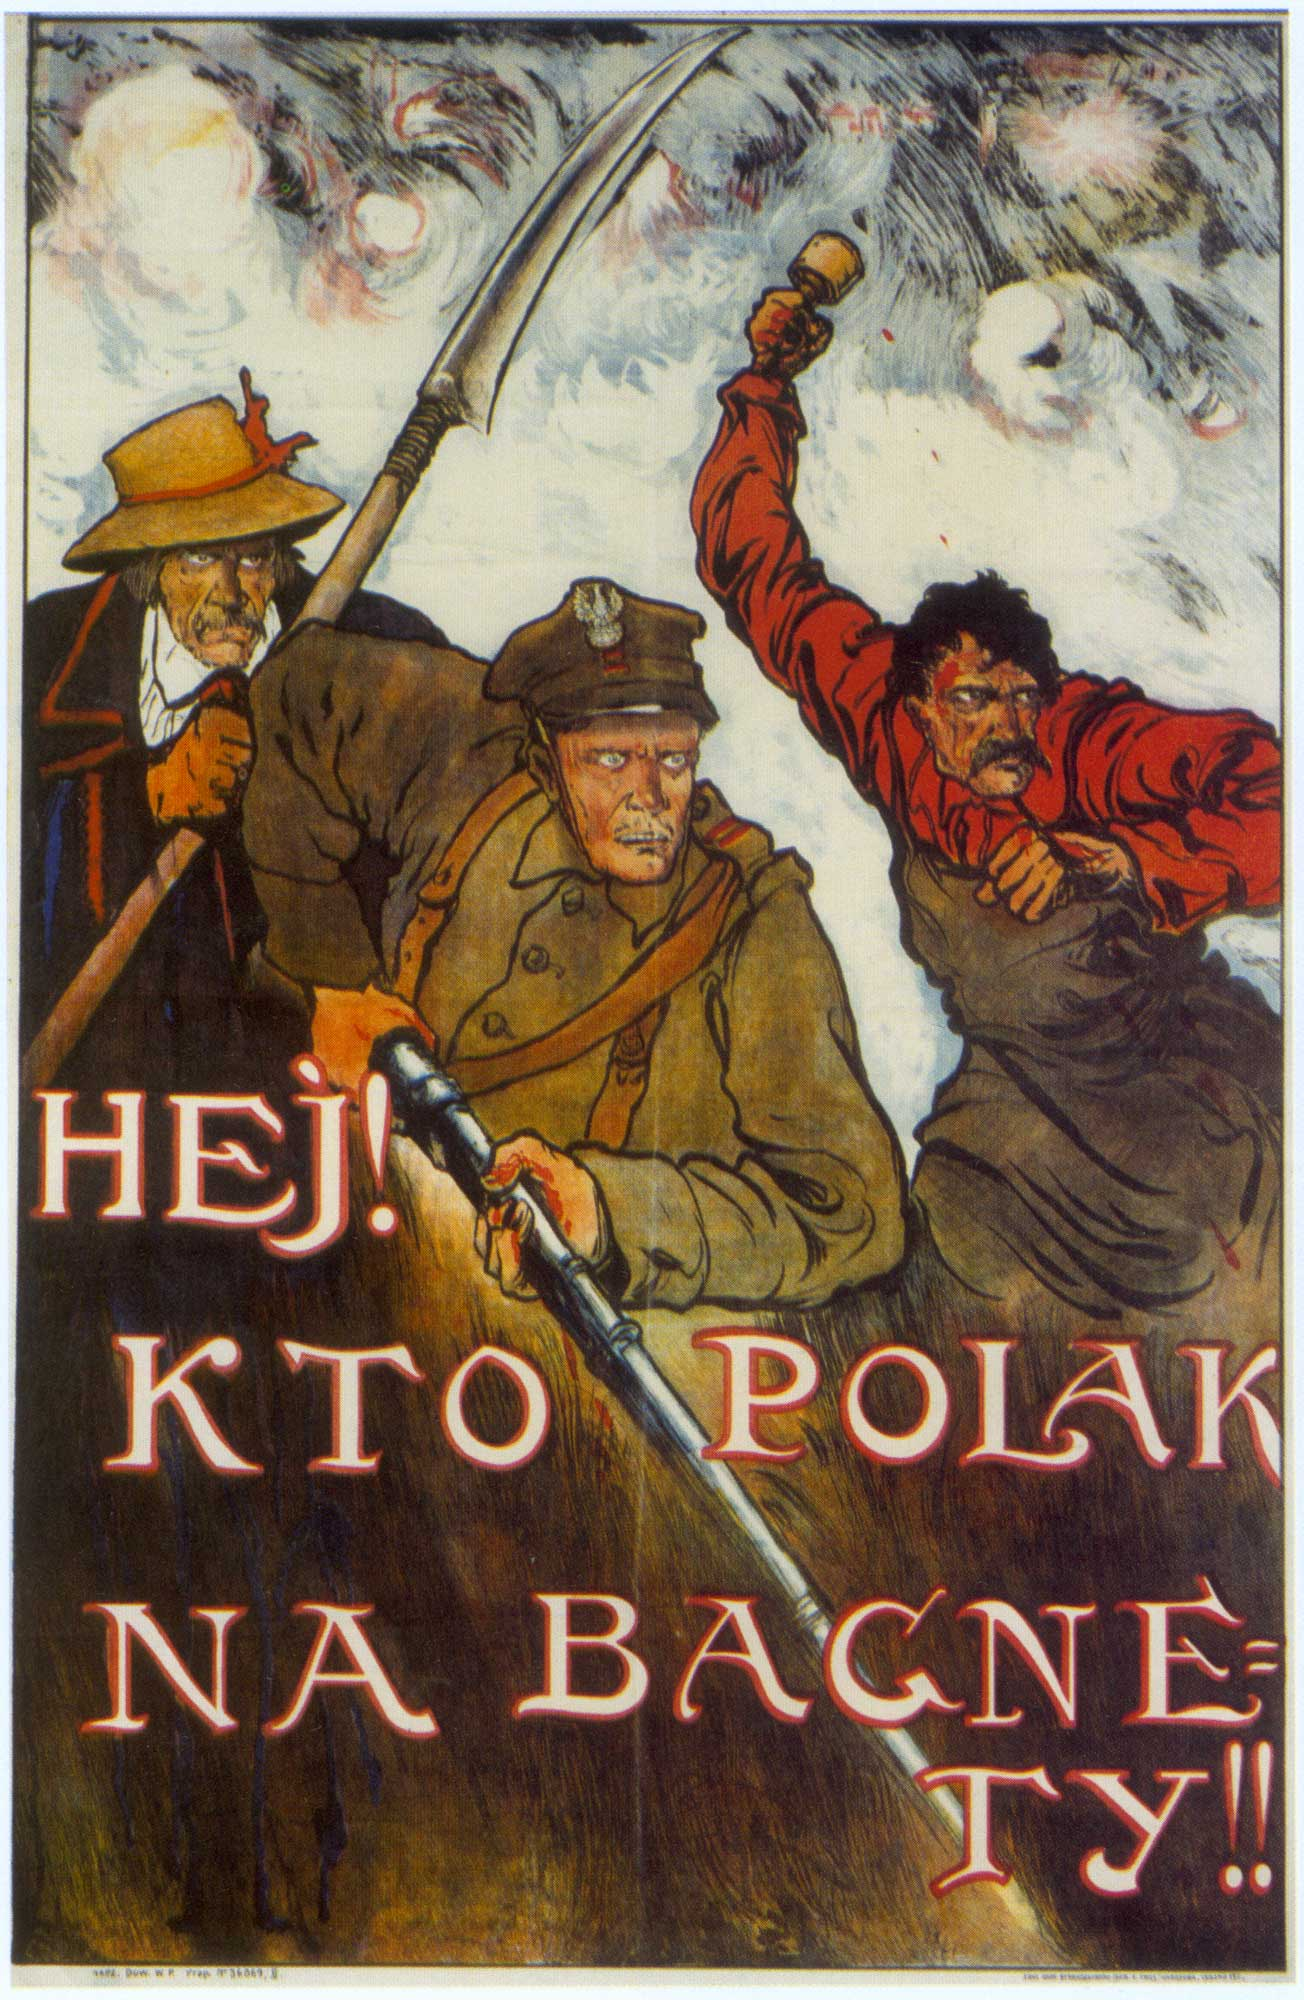
\includegraphics[width=0.35\paperwidth]{images/Na_bagnety.jpg}
			\end{columns}
		\end{itemize}
	\end{frame}
	
	\begin{frame}
		\frametitle{\textbf{Страна к 1921 г.}}
		\centering
		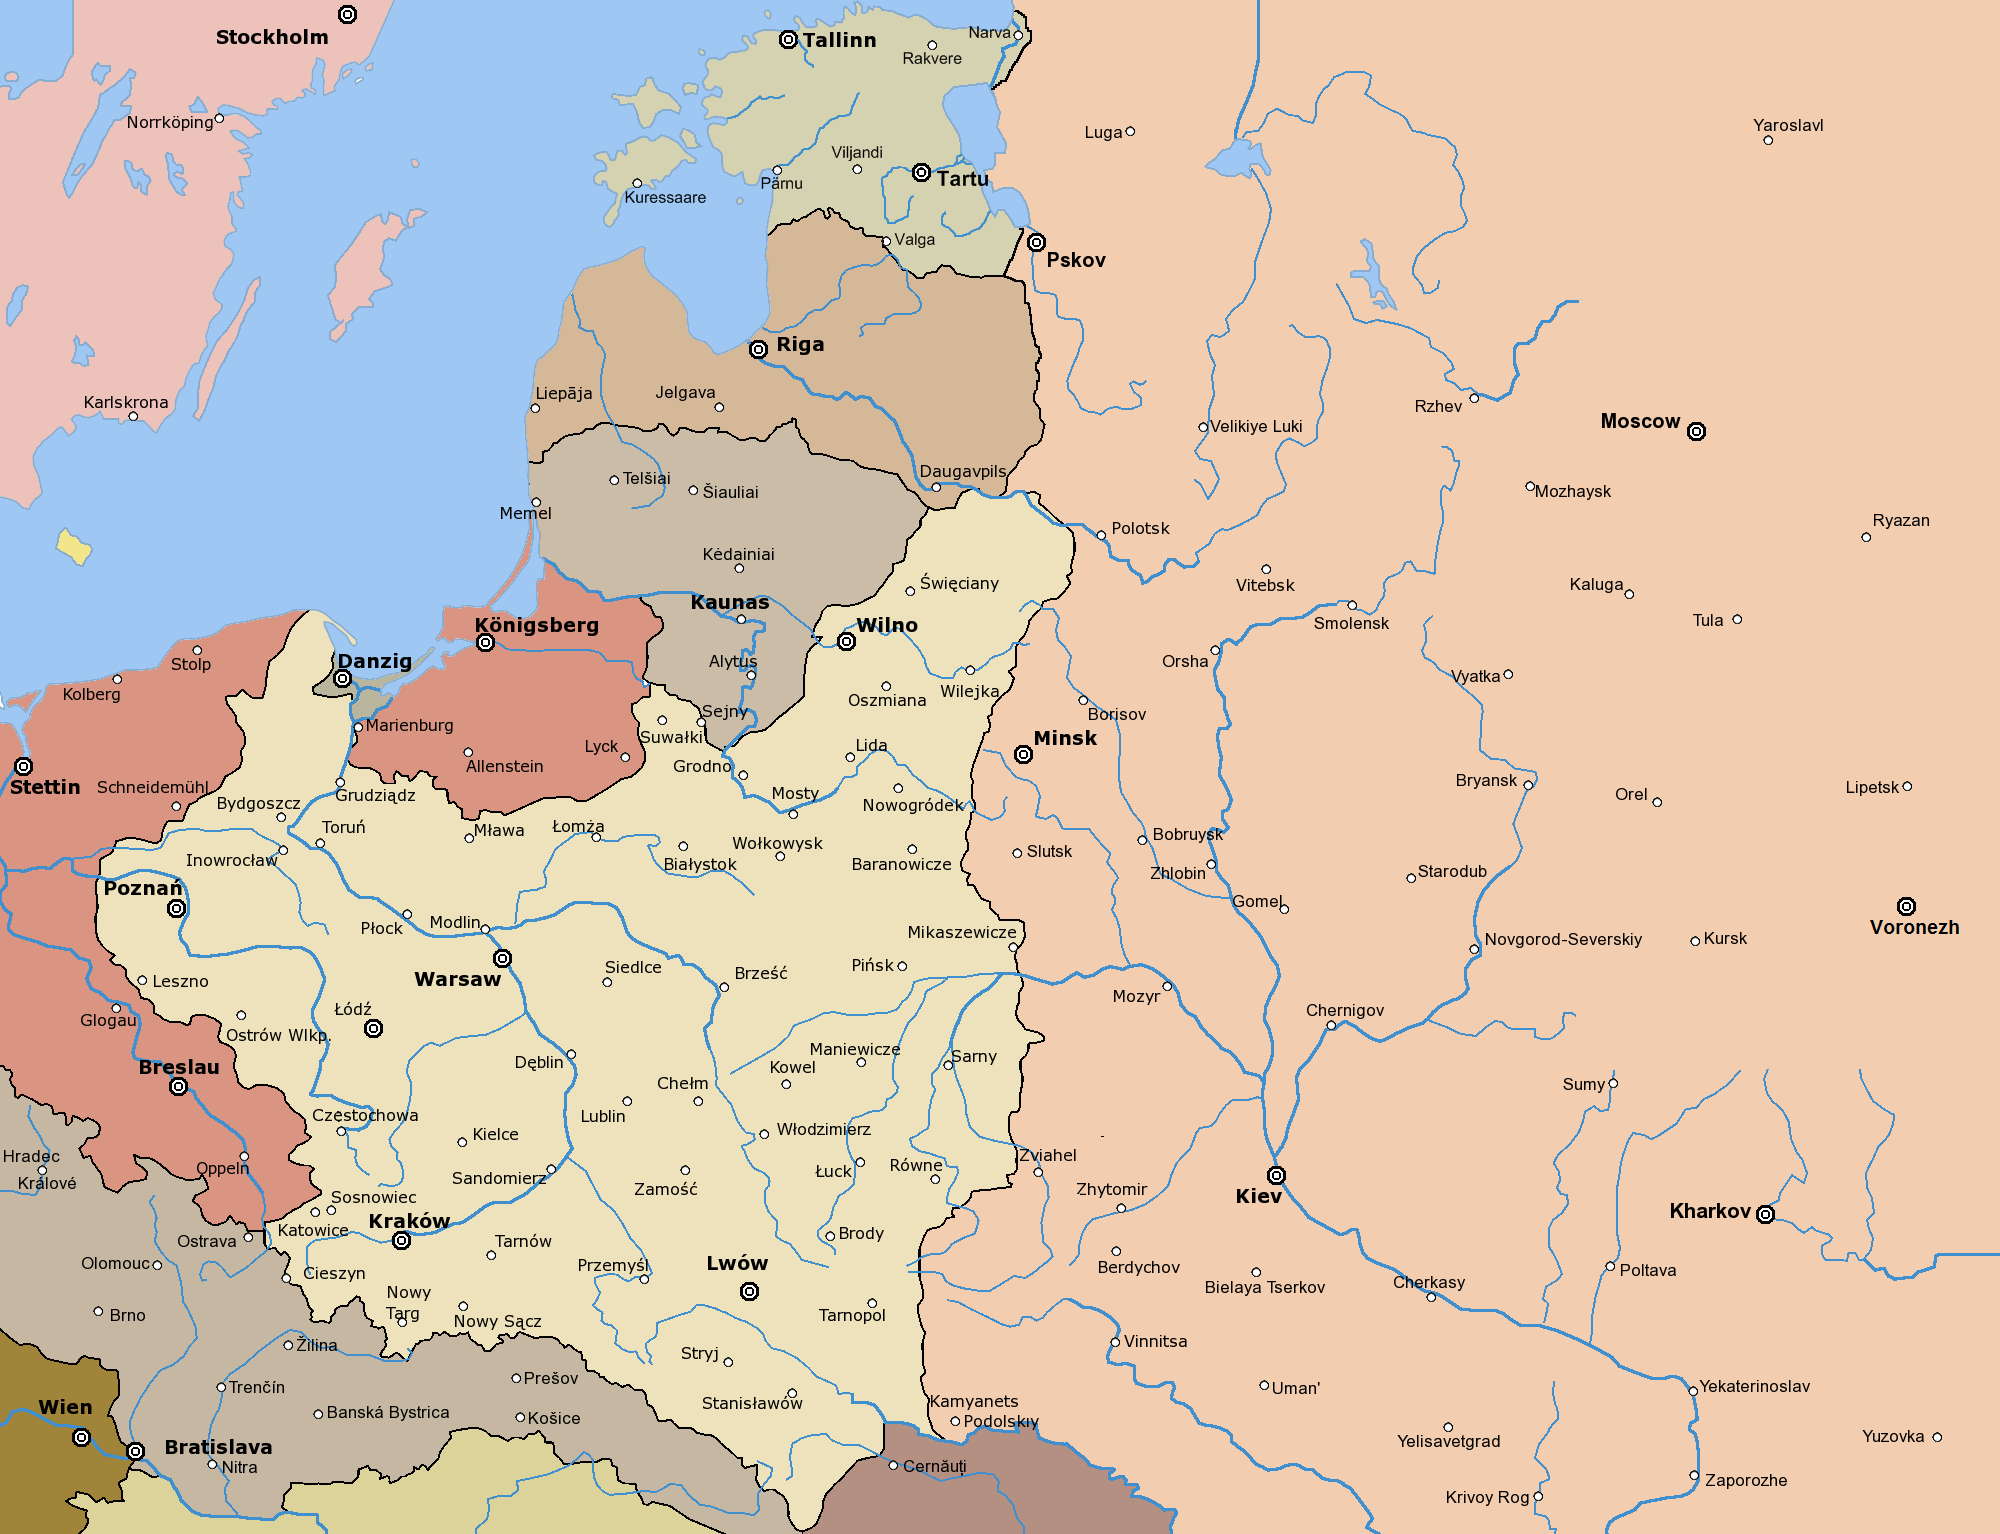
\includegraphics[width=0.8\paperwidth]{images/Rzeczpospolita_1923.png}
	\end{frame}
	
	\begin{frame}
		\frametitle{\textbf{Внутреннее устройство}}
		\begin{columns}[T] % T - выравнивание по верхнему краю
			\column{0.5\textwidth}
			В 1921 году была принята так называемая Мартовская конституция, установившая:
			\begin{itemize}
				\item сильный парламент (Сейм)
				\item слабую президентскую власть
				\item многопартийную систему
			\end {itemize}
			
			\column{0.5\textwidth}
			\centering
			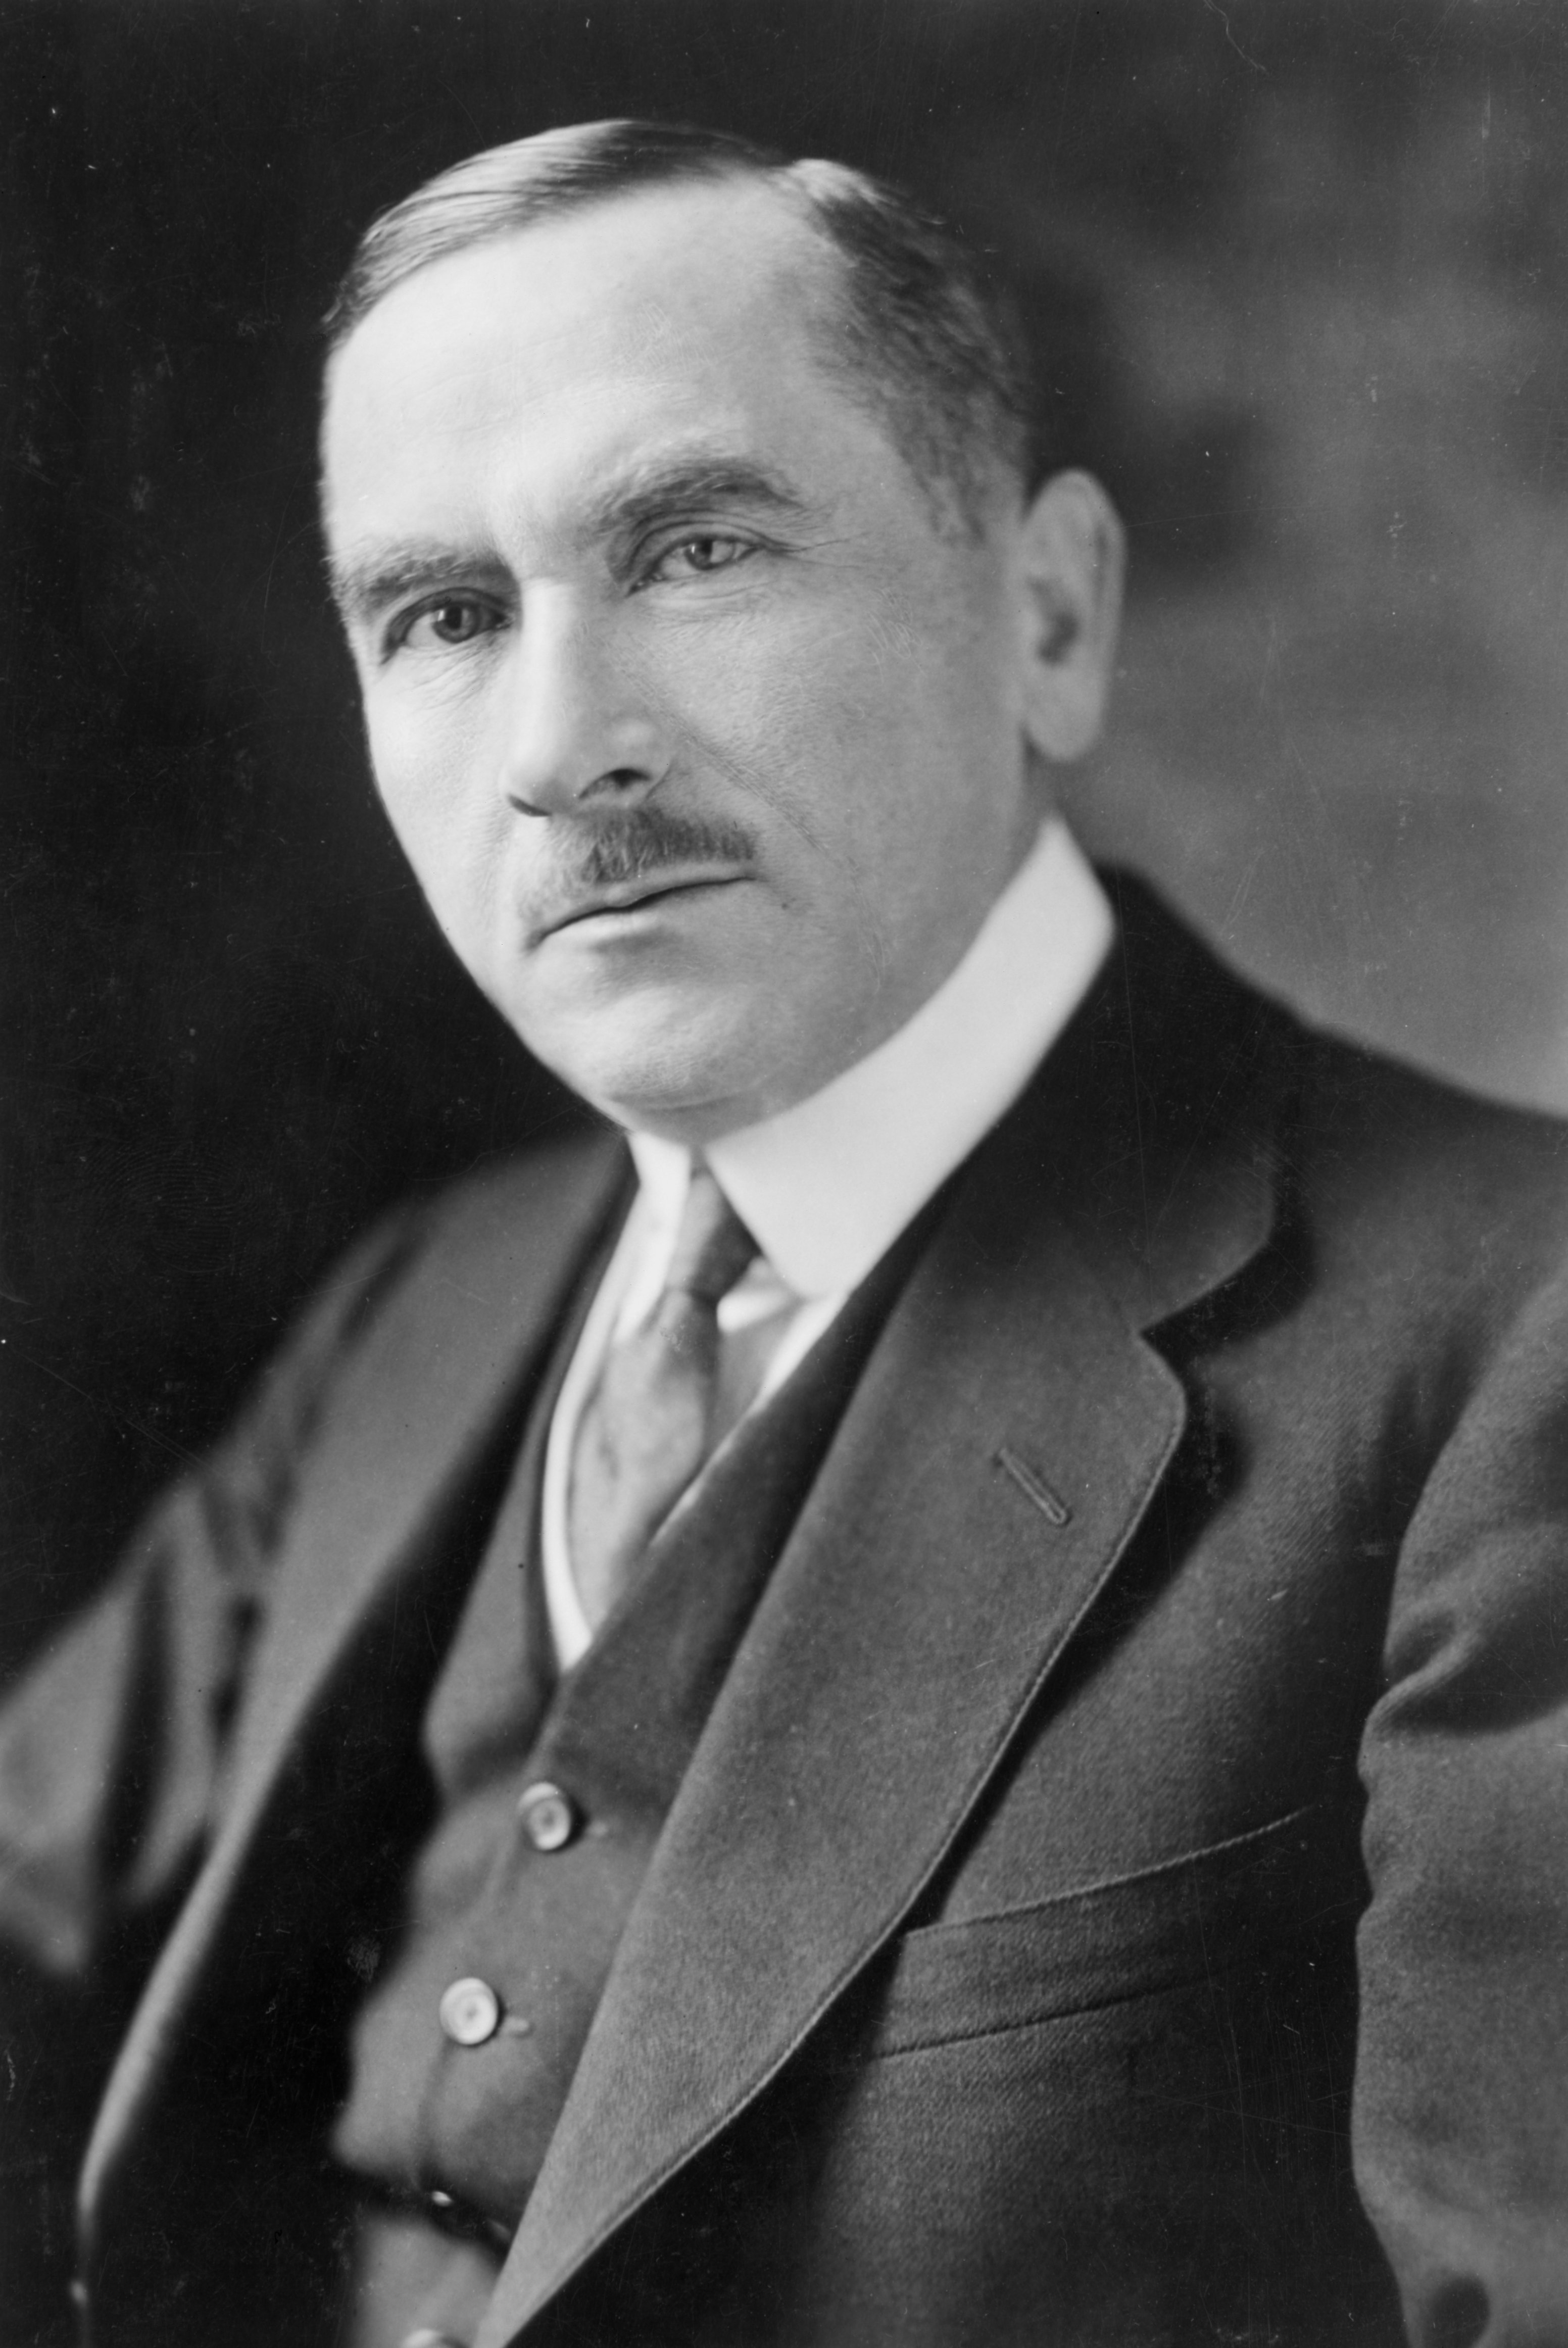
\includegraphics[width=0.35\paperwidth]{images/Roman_Dmowski_LOC_3c35372u.jpg}
			Ро́ман Стани́слав Дмо́вский \newline  9 августа 1864 —  2 января 1939
		\end{columns}
	\end{frame}
	
	\begin{frame}
		\frametitle{\textbf{Майский переворот 1926 года}}
		
		\begin{columns}[T] 
			\column{0.5\textwidth}
			Почему?
			\begin{itemize}
				\item Частая смена правительств
				\item Обвинения в коррупции
				\item Экономические трудности
				\item Страх перед "разложением государства"
			\end{itemize}
			
			\column{0.5\textwidth}
			\centering
			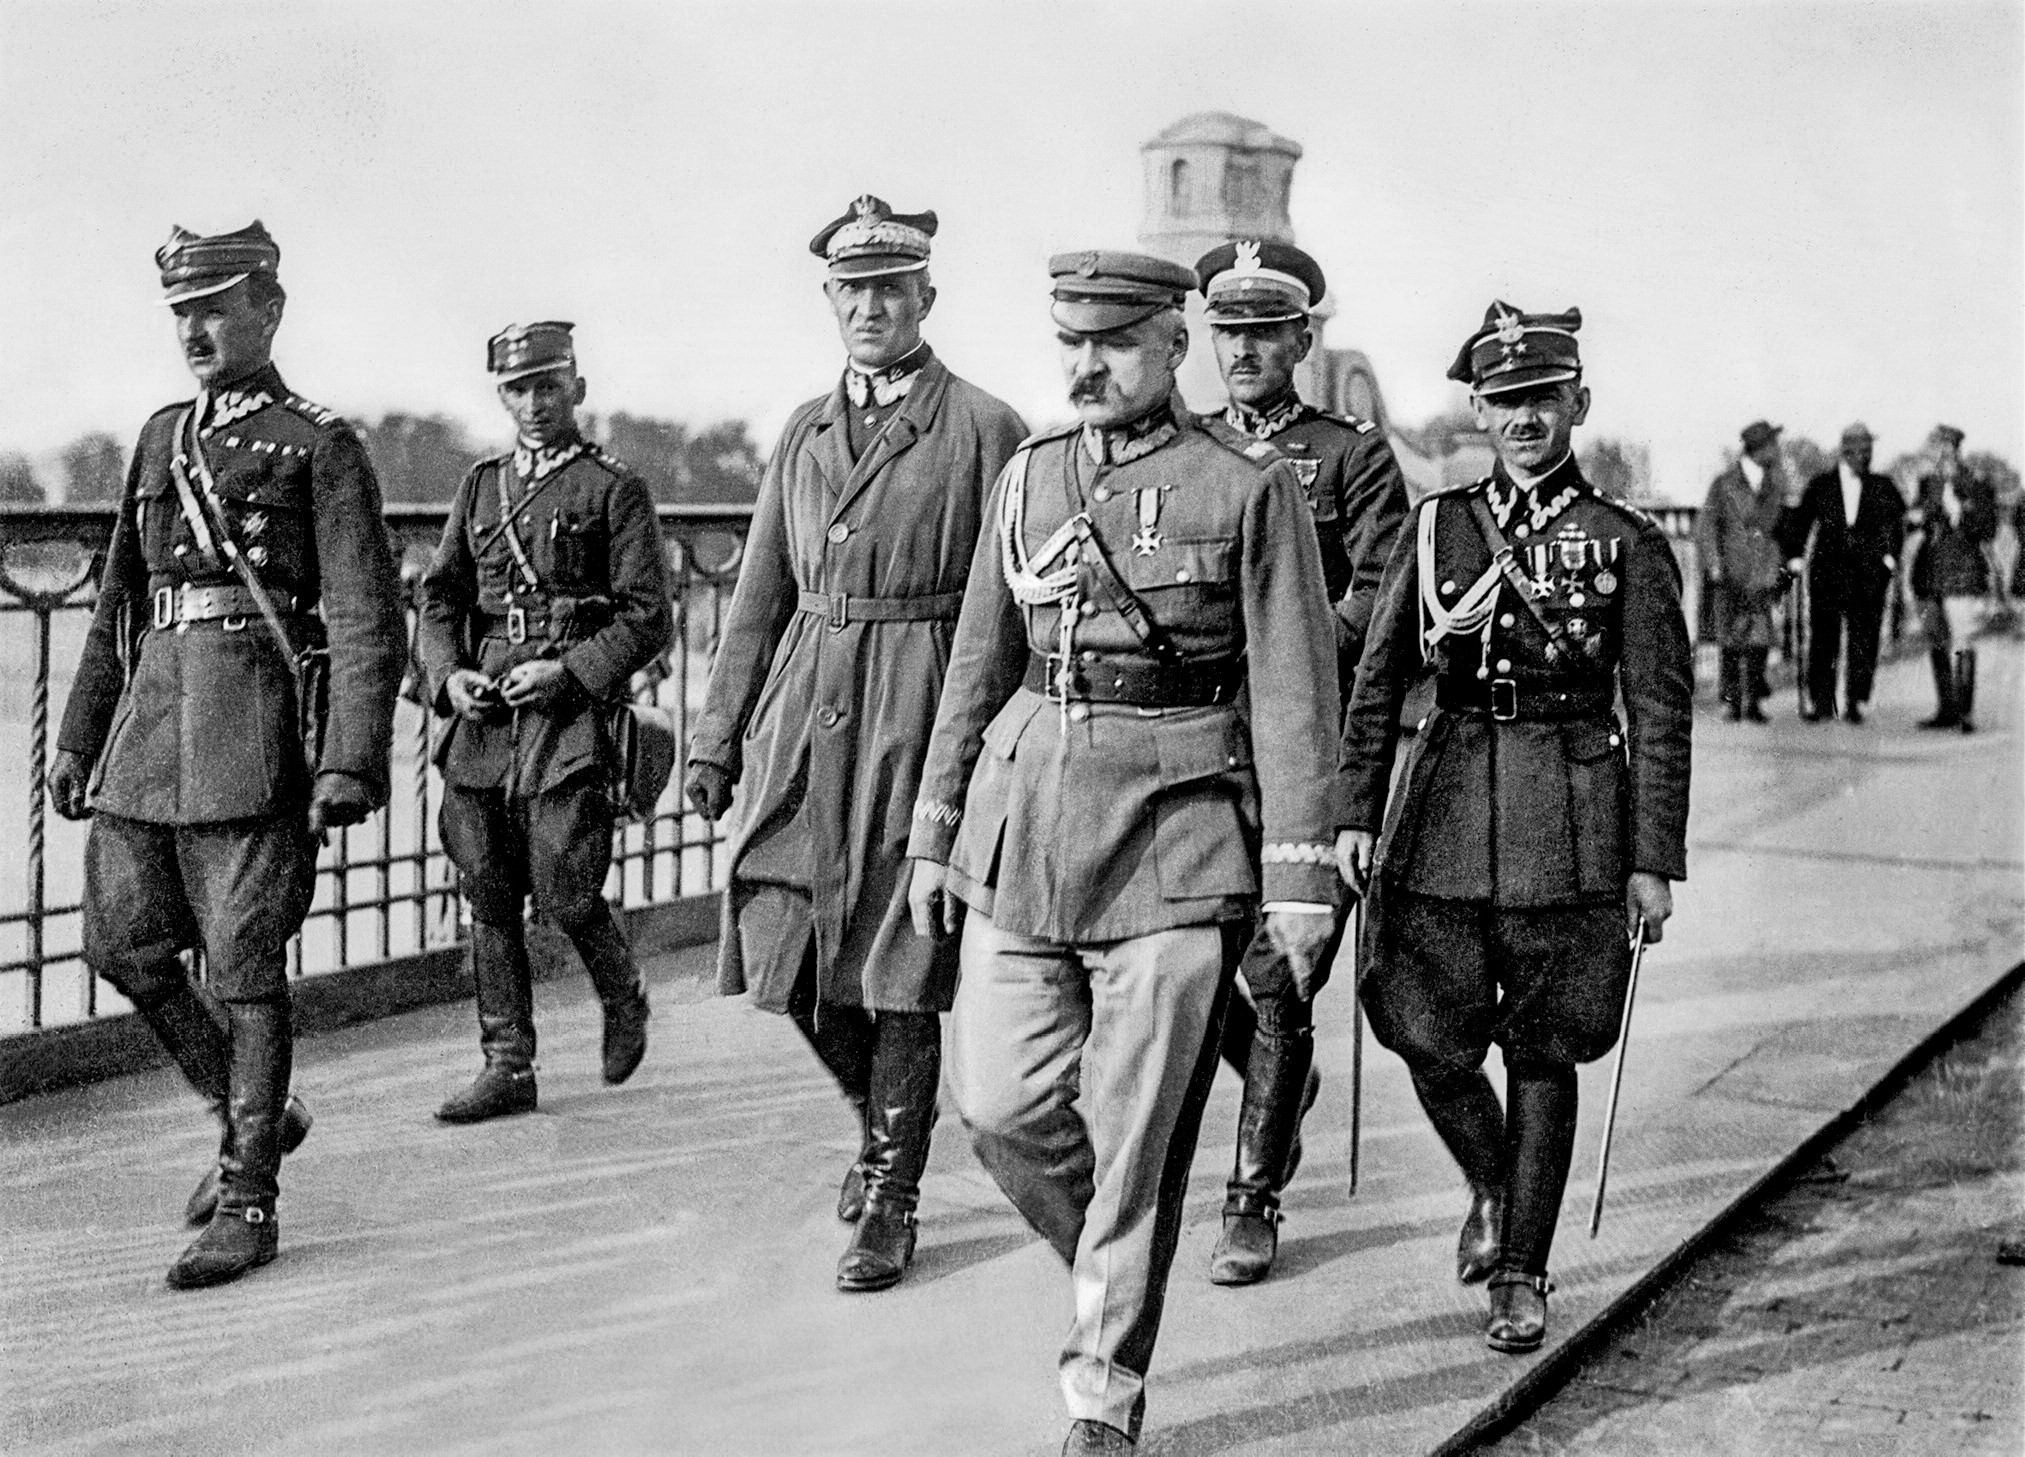
\includegraphics[width=\textwidth]{images/Piłsudski_May_1926.jpg}
			Пилсудский перед встречей с президентом Войцеховским на мосту Понятовского
		\end{columns}
	\end{frame}
	
	
	\begin{frame}
		\frametitle{\textbf{Кризис после смерти Пилсудского}}
		
		\begin{columns}[T] 
			\column{0.5\textwidth}
			\begin{itemize}
				\item Усиление внутриэлитной борьбы
				\item Рост национализма
				\item Режим Санации становится более консервативным и менее гибким
			\end{itemize}
			
			\column{0.5\textwidth}
			\centering
			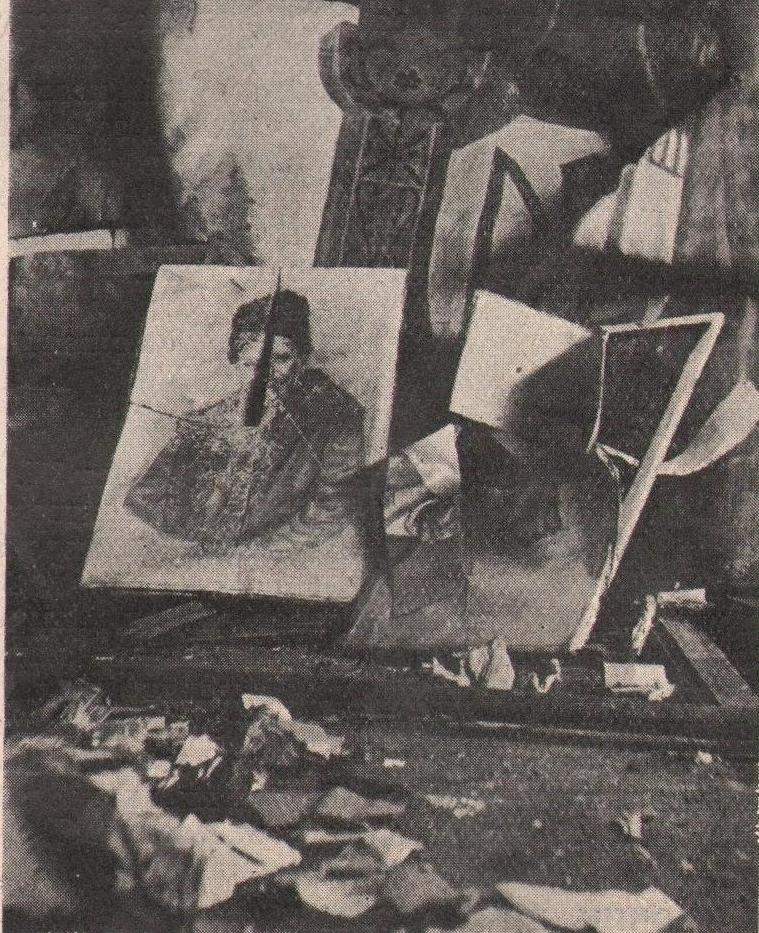
\includegraphics[width=\textwidth]{images/PACIF01.jpg}
		\end{columns}
	\end{frame}
	
\end{document}